\documentclass[12pt]{standalone}
\usepackage{tikz}

\begin{document}
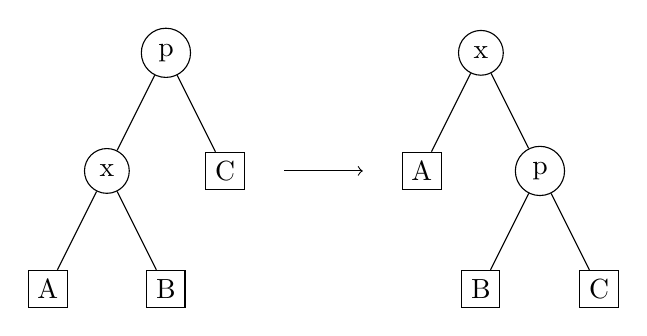
\begin{tikzpicture}

\tikzstyle{nodebase}=[align=center, text centered, draw]
\tikzstyle{node_a}=[nodebase, circle]
\tikzstyle{subtree}=[nodebase, rectangle]

\node [node_a] at (-2,0) {p}
    child {node [node_a] {x}
        child {node [subtree] {A}}
        child {node [subtree] {B}}}
    child {node [subtree] {C}};

\node [node_a] at (2,0) {x}
    child {node [subtree] {A}}
    child {node [node_a] {p}
        child {node [subtree] {B}}
        child {node [subtree] {C}}};

\draw[->] (-0.5,-1.5) -- ++(1,0);

\end{tikzpicture}
\end{document}
